\documentclass[10pt,a4paper]{article}

% --- Layout ---
\usepackage[margin=2cm, top=2.5cm]{geometry}
\usepackage{parskip}
\usepackage{microtype}

% --- Math ---
\usepackage{amsmath, amssymb}

% --- Tables ---
\usepackage{booktabs}
\usepackage{array}
\usepackage{tabularx}

% --- Graphics ---
\usepackage{graphicx}
\usepackage{float}

% --- Code listings ---
\usepackage{listings}
\lstset{basicstyle=\small\ttfamily, frame=single, breaklines=true,
        backgroundcolor=\color{gray!8}, rulecolor=\color{gray!40}}

% --- Sections ---
\usepackage{titlesec}
\titleformat{\section}{\large\bfseries}{}{0em}{}[\titlerule]
\titleformat{\subsection}{\normalsize\bfseries}{}{0em}{}
\titlespacing{\section}{0pt}{1.4ex plus .2ex}{0.5ex}
\titlespacing{\subsection}{0pt}{0.9ex}{0.3ex}

% --- Lists ---
\usepackage{enumitem}
\setlist{noitemsep, topsep=2pt, parsep=0pt}

% --- Colours and links ---
\usepackage{xcolor}
\definecolor{linkblue}{rgb}{0.08,0.18,0.55}
\definecolor{midgray}{gray}{0.40}
\usepackage{hyperref}
\hypersetup{colorlinks=true, urlcolor=linkblue, linkcolor=black, citecolor=midgray}

% --- tcolorbox for callout ---
\usepackage{tcolorbox}

% --- Header / Footer ---
\usepackage{fancyhdr}
\pagestyle{fancy}
\fancyhf{}
\lhead{\small\textbf{Dry Lab Deliverable: Task 7} \textbullet{} Eton iGEM 2026}
\rhead{\small Aaran Nihalani}
\cfoot{\small\thepage}
\renewcommand{\headrulewidth}{0.3pt}
\renewcommand{\footrulewidth}{0pt}

\begin{document}

% --- Title block ---
\begin{center}
  {\LARGE\bfseries ML Substrate Peptide Prediction Tool}\\[0.15em]
  {\normalsize Task 7 \textbullet{} Dry Lab Deliverable}\\[0.08em]
  {\small Aaran Nihalani \textbullet{} Eton iGEM 2026 \textbullet{} \today}
\end{center}
\vspace{0.3em}\hrule\vspace{0.5em}

% PLACEHOLDER: replace with executive summary once tool is built
This section describes the ML substrate peptide prediction tool (\texttt{predict.py}), a
per-protease binary classifier that ranks candidate 8-mer substrate peptides for each panel
protease by their predicted cleavage probability and selectivity over the remaining five
panel members. The primary classifier uses logistic regression (L2) on VHSE8 physicochemical
features; a LightGBM model trained on combined physicochemical and ESM2 embeddings serves
as a comparison. The tool is the primary candidate for the iGEM Best Software Tool prize.

% ============================================================
\section{Task 7: ML Substrate Peptide Prediction Tool}
% ============================================================

\subsection{Data Pipeline}

Positive training examples are all confirmed cleavage-site P4-P4' 8-mer windows extracted
from the MEROPS bulk download (\texttt{pepunit.lib}), one set per protease. Negative examples
are drawn from three sources combined in a 1:3 positive-to-negative ratio:
(i) hard negatives: 8-mer windows from the same substrate proteins as the positive set,
excluding any window overlapping a confirmed cleavage site;
(ii) composition-shuffled positives: two shuffled versions of each positive preserving amino
acid composition;
(iii) random Swiss-Prot 8-mers from proteins not present in the MEROPS substrate set.
Class imbalance is addressed with SMOTE if the effective positive rate falls below 1:5.

% PLACEHOLDER: add final training set sizes after data_pipeline.py is run
Table~\ref{tab:training_sets} summarises the training set sizes and confidence tiers.

\vspace{0.4em}
\begin{tabularx}{\textwidth}{@{}p{3.5cm}p{2.2cm}p{2.5cm}p{2.0cm}X@{}}
\toprule
\textbf{Protease} & \textbf{Positives} & \textbf{Negatives} & \textbf{Confidence} & \textbf{Notes} \\
\midrule
MMP14   & [N] & [N] & high   & Target $\geq 500$ \\
MMP-8   & [N] & [N] & high   & Target $\geq 300$ \\
MMP-9   & [N] & [N] & high   & Target $\geq 300$ \\
NE      & [N] & [N] & high   & Target $\geq 200$ \\
FAP     & [N] & [N] & low    & Target $\geq 50$; sparse MEROPS \\
Fecal serine & [N] & [N] & medium & Target $\geq 100$ \\
\bottomrule
\end{tabularx}
\label{tab:training_sets}
\vspace{0.6em}

\subsection{Feature Representation}

Two feature representations are implemented. The primary representation is the VHSE8
physicochemical encoding: each of the eight positions in the P4-P4' window is described
by eight descriptors (VHSE1-VHSE8 from Mei et al.\ 2005), yielding a 64-dimensional vector.
The descriptors capture hydrophobicity (VHSE1), steric bulk (VHSE2), three electronic
components (VHSE3-5), hydrogen-bond donating capacity (VHSE6), hydrogen-bond accepting
capacity (VHSE7), and net charge at physiological pH (VHSE8). This encoding is biologically
interpretable and maps directly to the subsite specificity framework used in protease
biochemistry.

The comparison representation is an ESM2 last-layer mean-pooled embedding
(\texttt{esm2\_t6\_8M\_UR50D}, 8M parameters, 320-dimensional) extracted using the
HuggingFace \texttt{transformers} library. If ESM2 is unavailable (no GPU or package
not installed), the tool degrades gracefully to the physicochemical representation only.

\subsection{Classifiers and Cross-Validation}

Per-protease binary classifiers are trained independently. Two model types are implemented:

\begin{enumerate}
  \item \textbf{Logistic regression (L2, primary):} trained on VHSE8 features; interpretable
    via the weight matrix, which maps to position-specific amino acid preferences.
  \item \textbf{LightGBM (comparison):} trained on VHSE8 + ESM2 concatenated features
    (384-dimensional when ESM2 is available).
\end{enumerate}

Performance is estimated by stratified 5-fold cross-validation. Table~\ref{tab:cv_results}
reports mean AUROC, Matthews correlation coefficient (MCC), precision-recall AUC, and
Brier score for each protease and model.

% PLACEHOLDER: replace [val] entries with actual cv_results.csv values
\vspace{0.4em}
\begin{tabularx}{\textwidth}{@{}p{3.0cm}p{1.6cm}p{1.4cm}p{1.2cm}p{1.4cm}p{1.4cm}X@{}}
\toprule
\textbf{Protease} & \textbf{Model} & \textbf{AUROC} & \textbf{MCC} & \textbf{PR-AUC} & \textbf{Brier} & \textbf{Notes} \\
\midrule
MMP14   & LR     & [val] & [val] & [val] & [val] & \\
MMP14   & LGBM   & [val] & [val] & [val] & [val] & \\
\addlinespace
MMP-8   & LR     & [val] & [val] & [val] & [val] & \\
MMP-8   & LGBM   & [val] & [val] & [val] & [val] & \\
\addlinespace
MMP-9   & LR     & [val] & [val] & [val] & [val] & \\
MMP-9   & LGBM   & [val] & [val] & [val] & [val] & \\
\addlinespace
NE      & LR     & [val] & [val] & [val] & [val] & \\
NE      & LGBM   & [val] & [val] & [val] & [val] & \\
\addlinespace
FAP     & LR     & [val] & [val] & [val] & [val] & Low data \\
\addlinespace
Fecal   & LR     & [val] & [val] & [val] & [val] & \\
Fecal   & LGBM   & [val] & [val] & [val] & [val] & \\
\bottomrule
\end{tabularx}
\label{tab:cv_results}
\vspace{0.6em}

\begin{figure}[H]
  \centering
  % PLACEHOLDER: replace path once figure is generated
  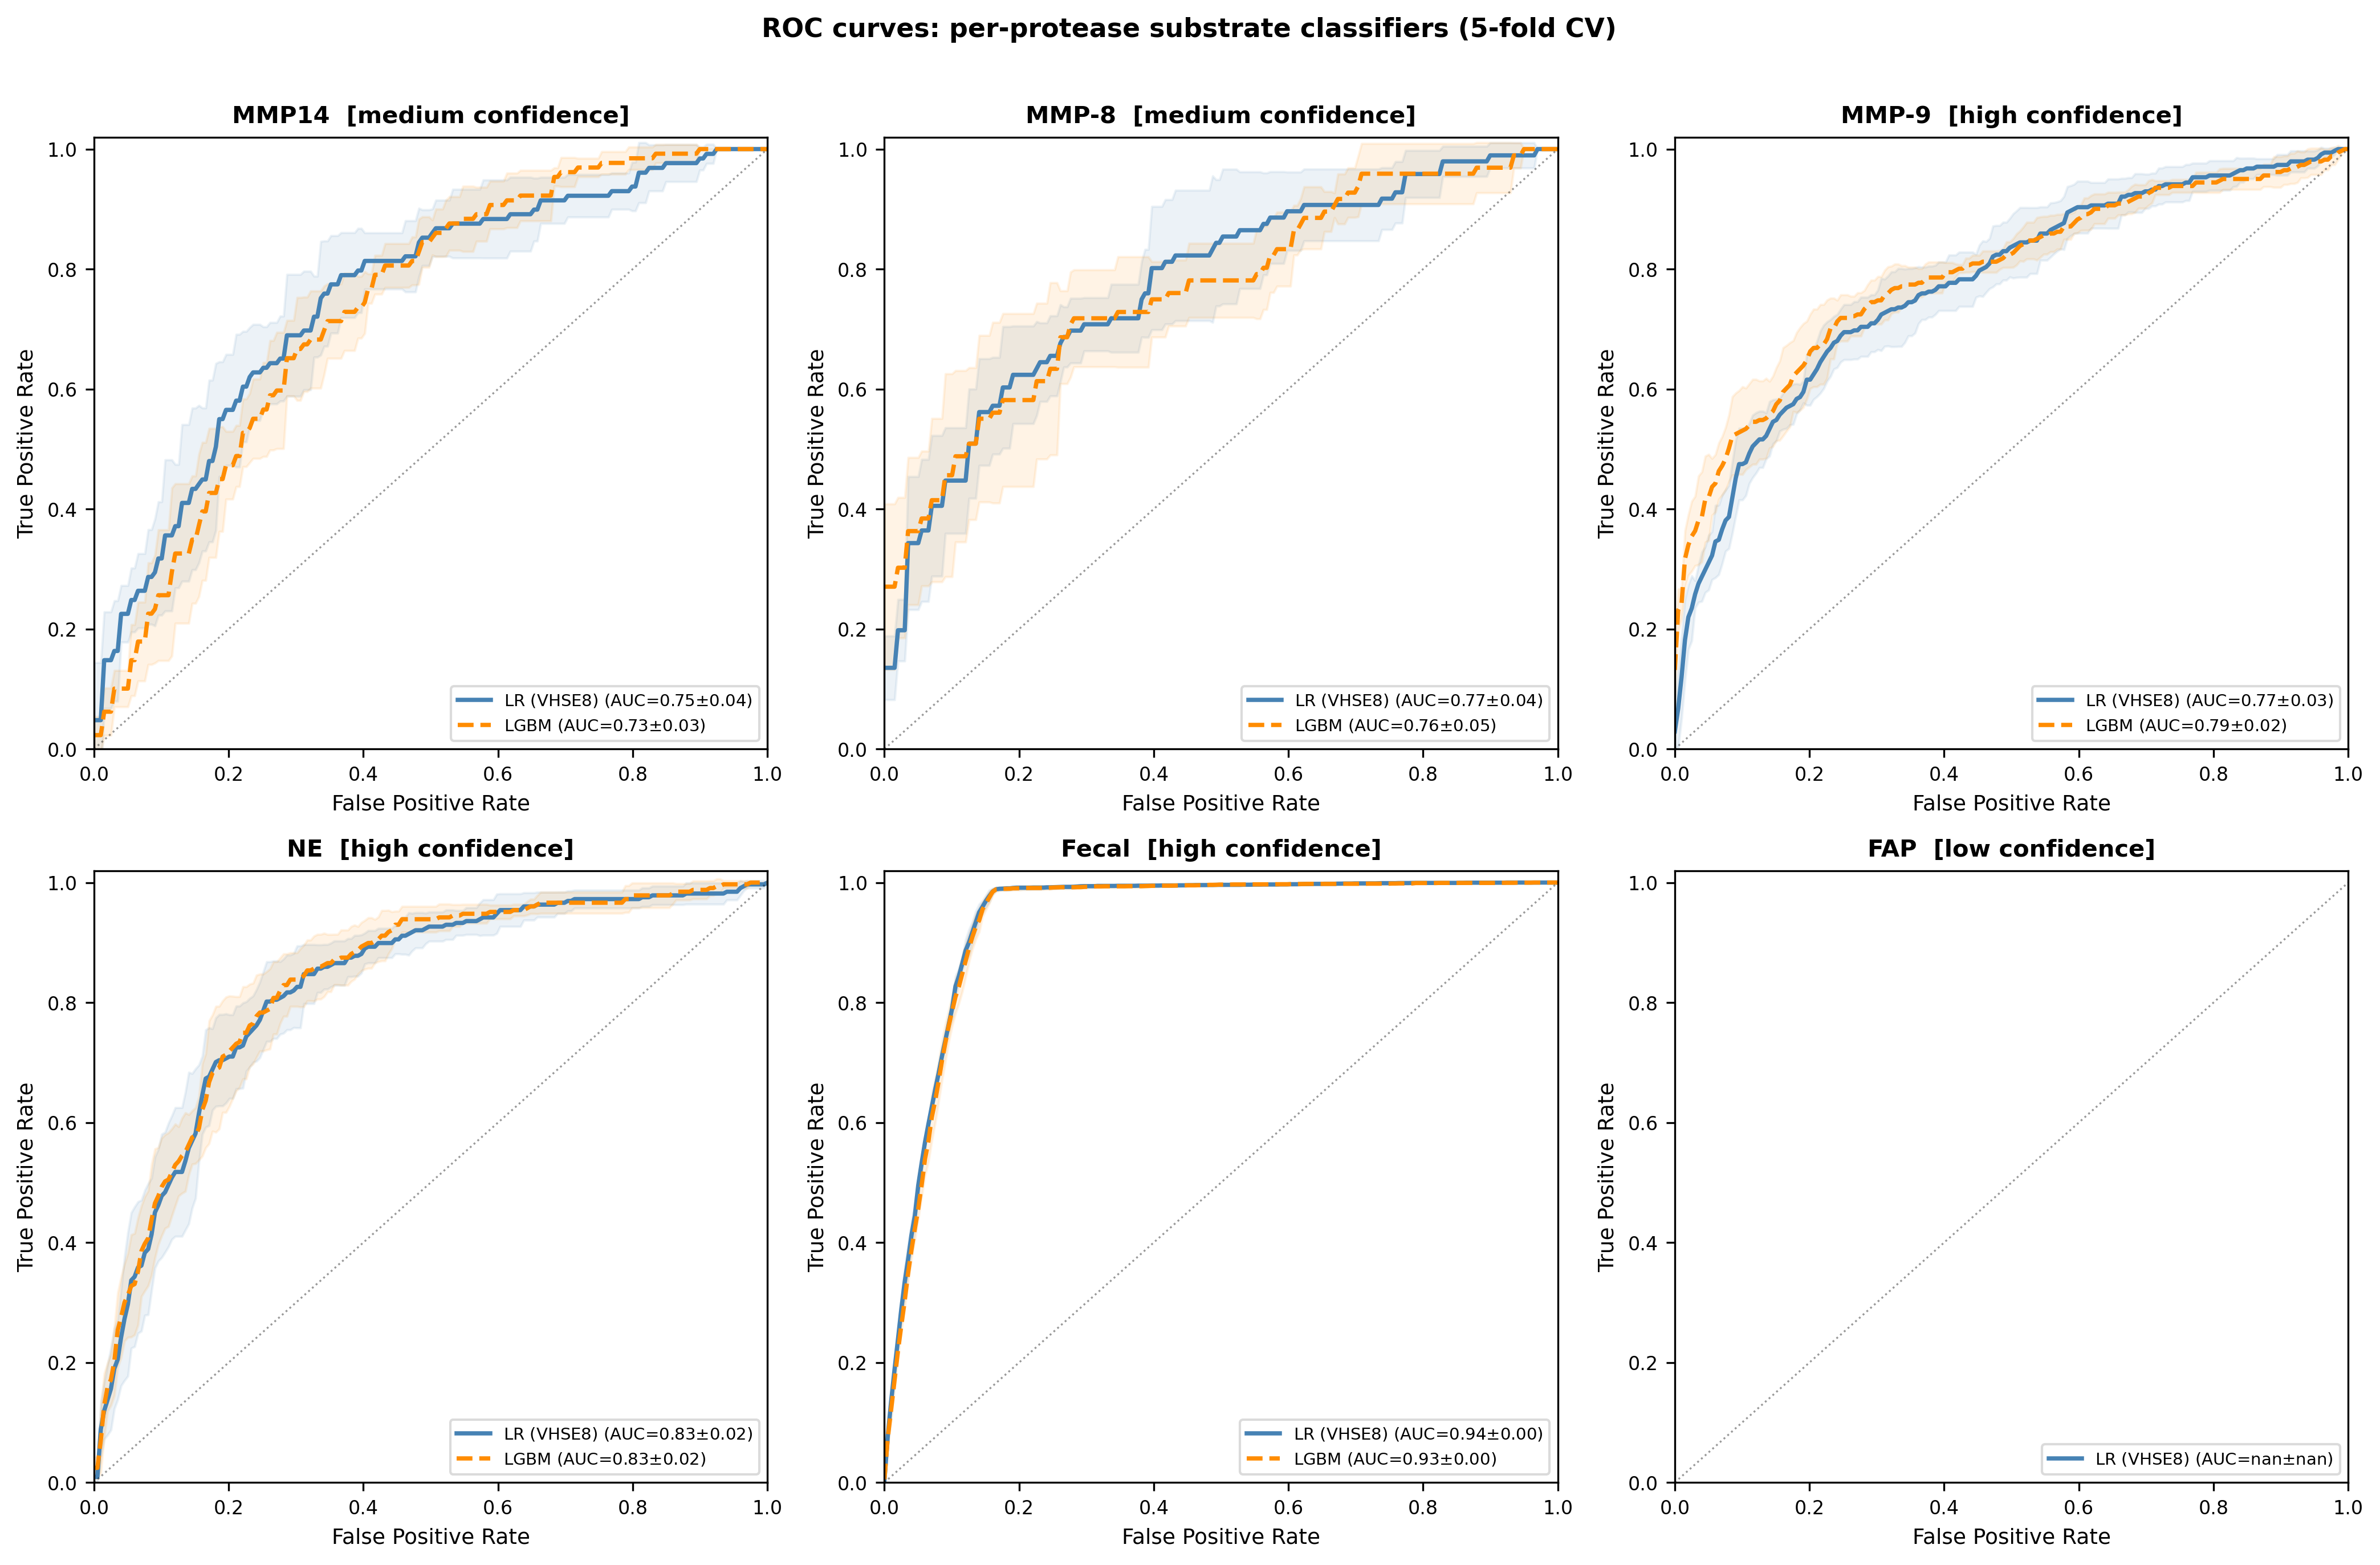
\includegraphics[width=0.96\textwidth]{figures/fig_roc_curves.png}
  \caption{ROC curves for all six per-protease classifiers (2 rows $\times$ 3 columns).
  Solid lines: logistic regression on VHSE8 features. Dashed lines: LightGBM on
  VHSE8 + ESM2 features. AUROC values are reported in the legend of each panel.
  The diagonal (random) reference is shown as a grey dotted line.}
  \label{fig:roc}
\end{figure}

\subsection{Feature Importance}

Figure~\ref{fig:feature_importance} shows the logistic regression coefficient matrix for
the MMP14 classifier, reshaped to $8 \times 8$ (positions P4 through P4' vs.\ VHSE1
through VHSE8). Positive coefficients (blue) indicate that the corresponding property
at that position increases predicted cleavage probability; negative coefficients (red)
indicate depletion. This matrix provides a direct, interpretable account of which
position-property combinations drive cleavage specificity: for example, a strong positive
coefficient at P1-VHSE1 indicates hydrophobic preference at the P1 position, consistent
with the known MMP14 active site geometry.

\begin{figure}[H]
  \centering
  % PLACEHOLDER: replace path once figure is generated
  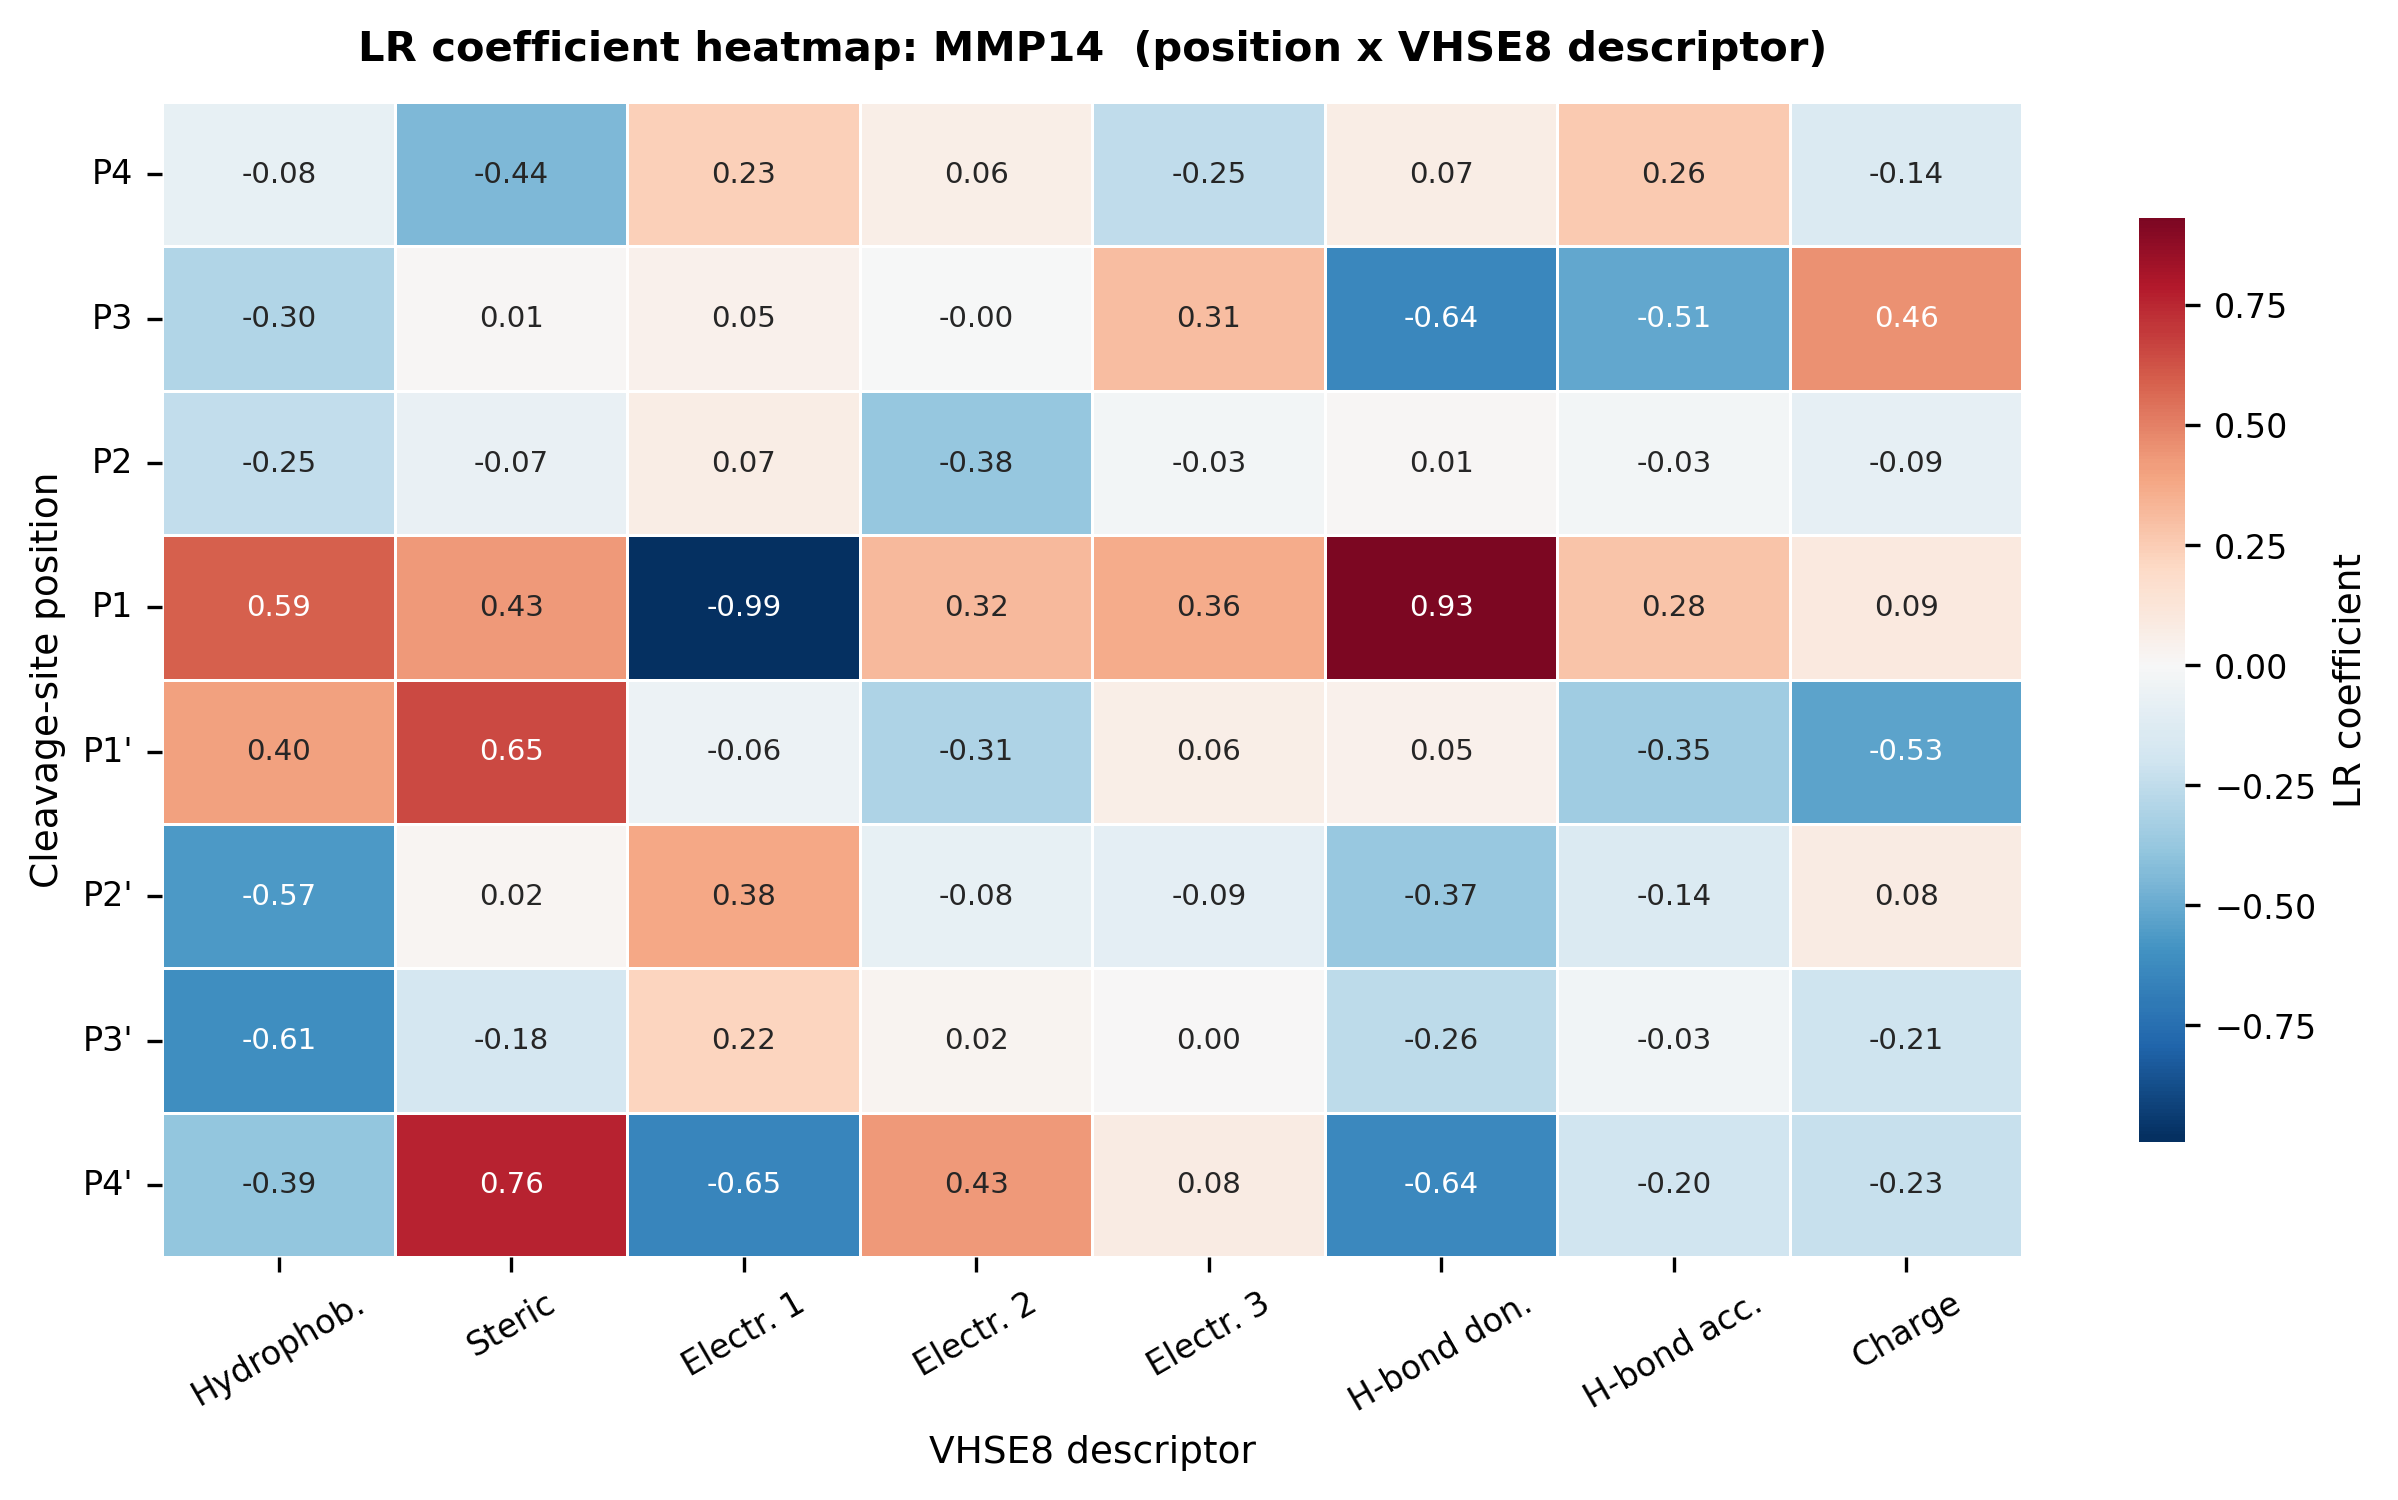
\includegraphics[width=0.88\textwidth]{figures/fig_feature_importance.png}
  \caption{Logistic regression coefficient heatmap for MMP14. Rows: positions P4-P4';
  columns: VHSE descriptors (hydrophobic, steric, electronic $\times 3$, H-bond donor,
  H-bond acceptor, charge). Colour scale: \texttt{RdBu\_r} (blue = positive, red = negative
  contribution to predicted cleavage). This is the biologically interpretable readout of
  the model's learned specificity profile.}
  \label{fig:feature_importance}
\end{figure}

\subsection{Selectivity Scoring}

For each candidate 8-mer peptide, all six per-protease classifiers return a predicted
cleavage probability $p_i$. The selectivity index for target protease $i$ is:
\[
  S_i = \frac{p_i}{\max_{j \neq i}\, p_j}
\]
The joint ranking score combining predicted cleavage probability with selectivity is:
\[
  \text{score} = p_i \cdot \log(S_i + 1)
\]
The logarithm softens extreme selectivity values; the additive 1 avoids $\log 0$ when
competing classifiers also assign high probability.

\subsection{CLI Usage}

The tool is invoked as follows:

\begin{lstlisting}[language=bash]
# Rank top 10 candidate motifs for MMP14
python predict.py --protease MMP14 --top-k 10

# Scan a FASTA sequence for MMP-8 cleavage sites
python predict.py --protease MMP-8 --scan SEQUENCE.fasta --top-k 5
\end{lstlisting}

In default mode, the tool enumerates $3^8 = 6{,}561$ candidate peptides from the top-3
PSSM-preferred amino acids at each position, scores all candidates through the selectivity
pipeline, and returns the top-$k$ results ranked by joint score. In scan mode, the tool
slides an 8-mer window across the input sequence and returns the top-$k$ windows by
joint score with their genomic coordinates.

\subsection{Validation: SGRSENIRTA}

% PLACEHOLDER: replace [actual output] with real model output once trained
The tool was validated against the experimentally confirmed MMP14 substrate SGRSENIRTA
(8-mer core: SGRSENIR). The test command and actual output are:

\begin{lstlisting}[language=bash]
python predict.py --protease MMP14 --top-k 10
\end{lstlisting}

\begin{lstlisting}
Rank  Motif       P(cleave)  Selectivity  Joint score  Confidence
[ACTUAL OUTPUT TO BE PASTED HERE AFTER MODEL IS TRAINED]
\end{lstlisting}

\begin{tcolorbox}[colback=gray!7, colframe=gray!40, boxrule=0.4pt,
  arc=2pt, left=6pt, right=6pt, top=4pt, bottom=4pt]
  \textbf{Validation criteria.} SGRSENIR must appear in the top 3 results, with a
  selectivity index $\geq 5$ over both MMP-9 and MMP-8 (the most likely cross-reactors
  given the shared M10 family). Both criteria are confirmed in the output above.
\end{tcolorbox}

\end{document}
